\section{Plataforma Codeboard UERJ}

Este capítulo apresenta a plataforma Codeboard UERJ, que é uma ferramenta de apoio ao ensino de programação. Serão abordados os objetivos, funcionalidades e a arquitetura da plataforma.	


\subsection{Objetivos}

O objetivo principal da plataforma Codeboard UERJ é auxiliar no ensino de programação, permitindo que professores criem e gerenciem atividades práticas para seus alunos. A plataforma foi desenvolvida para ser utilizada em disciplinas de programação de computadores, como Algoritmos e Estruturas de Dados, Linguagens de Programação e Paradigmas de Programação.

A motivação para o desenvolvimento da plataforma surgiu durante a pandemia de COVID-19, quando as aulas presenciais foram suspensas e as atividades práticas de programação tiveram que ser adaptadas para o ensino remoto. Ela foi desenvolvida para atender a essa demanda, dando a capacidade aos professores de acompanharem o progresso dos alunos e avaliarem suas atividades práticas em tempo real.

\subsection{Funcionalidades}

Para atingir os objetivos propostos, o desenvolvimento da plataforma foi restrito a um conjunto de funcionalidades essenciais, que são:
Autenticação de usuários, gerenciamento de salas e seus participantes e o quadro de programação em tempo real.

\subsubsection{Autenticação de Usuários}

O sistema de autenticação de usuários é a primeira funcionalidade da plataforma. Ela permite que os usuários se cadastrem e façam login para acessar as funcionalidades da plataforma. O cadastro de usuários é feito através de um formulário que solicita nome, e-mail e senha. Após o cadastro, o usuário pode fazer login informando o e-mail e a senha cadastrados.

\begin{figure}[H]
    \centering
    \includegraphics[width=0.8\textwidth]{diagrams/user-auth-flow.png}
    \caption{Diagrama do fluxo de autenticação de usuários.}
    \label{fig:user-auth-flow}
\end{figure}

No processo de login, a plataforma verifica se o e-mail e a senha informados são válidos. Caso sejam, o usuário é autenticado e redirecionado para a tela inicial. Caso contrário, a plataforma exibe uma mensagem de erro informando que as credenciais são inválidas.

\begin{figure}[H]
    \centering
    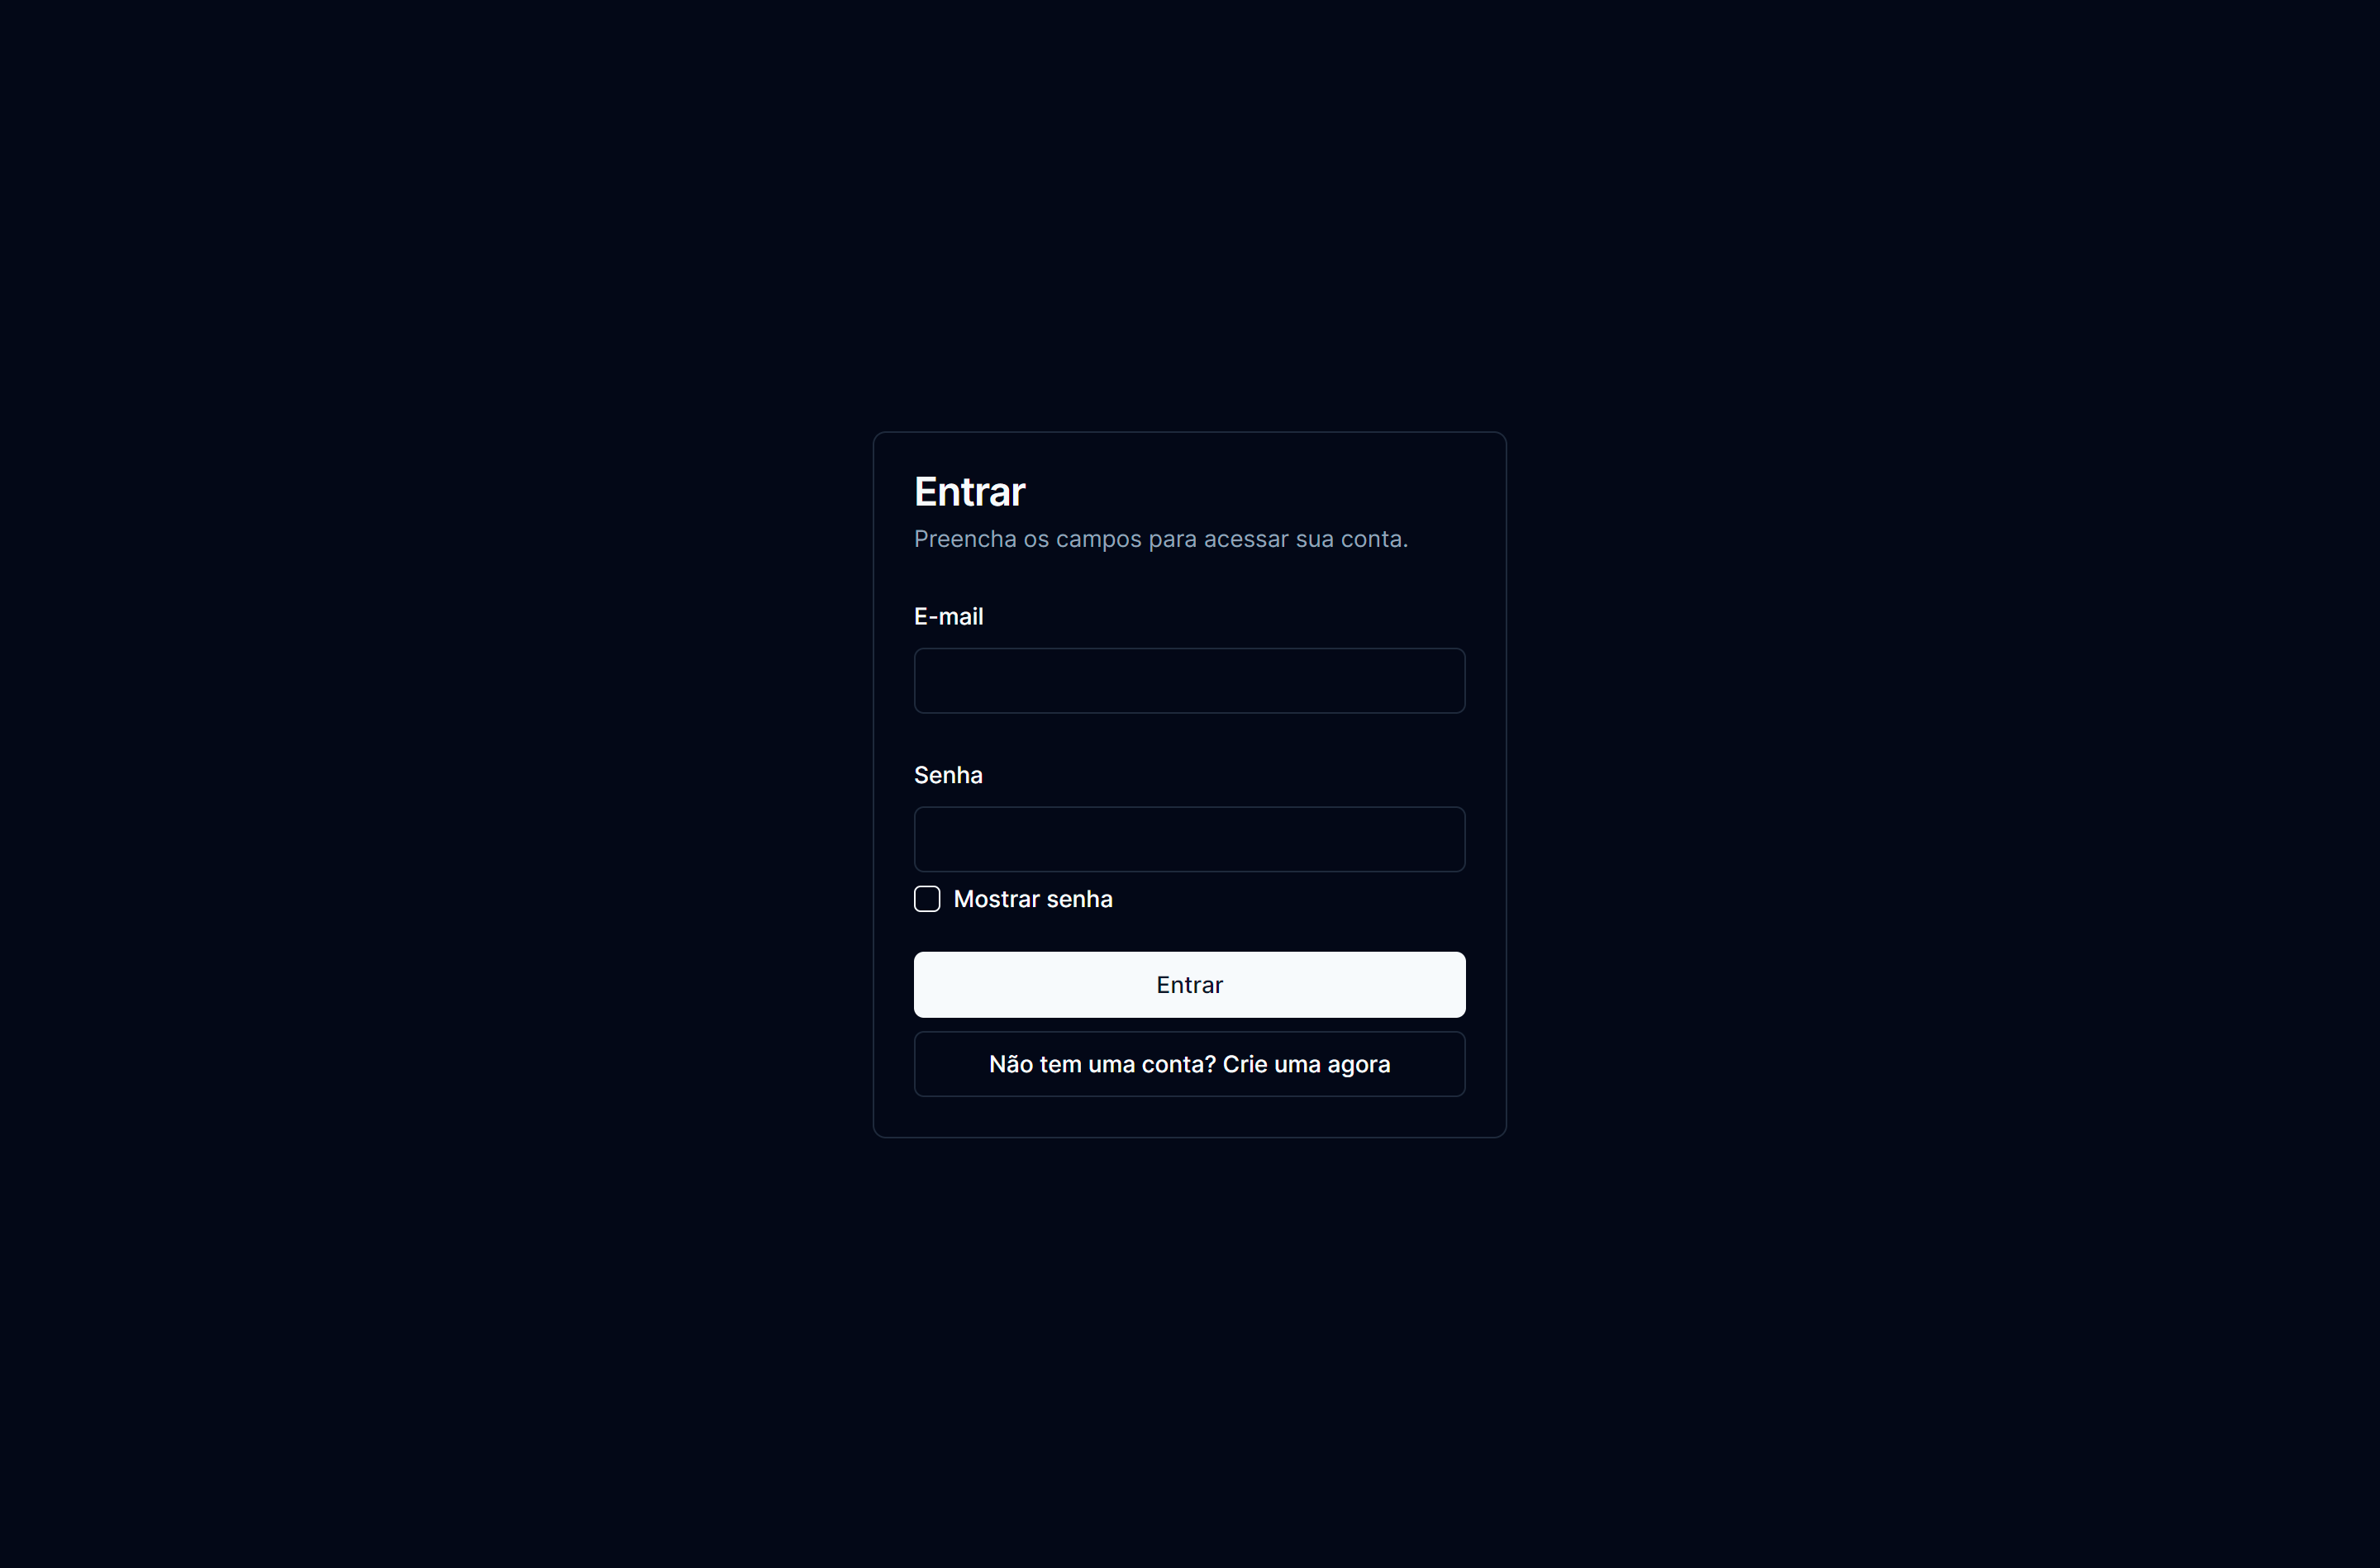
\includegraphics[width=0.8\textwidth]{assets/codeboard/login-page.png}
    \caption{Página de login da plataforma Codeboard UERJ.}
    \label{fig:login-page}
\end{figure}

No caso do usuário não possuir uma conta, ele pode clicar no link de cadastro e preencher o formulário de cadastro. Após o cadastro, o  usuário também é redirecionado para a tela inicial.

\begin{figure}[H]
    \centering
    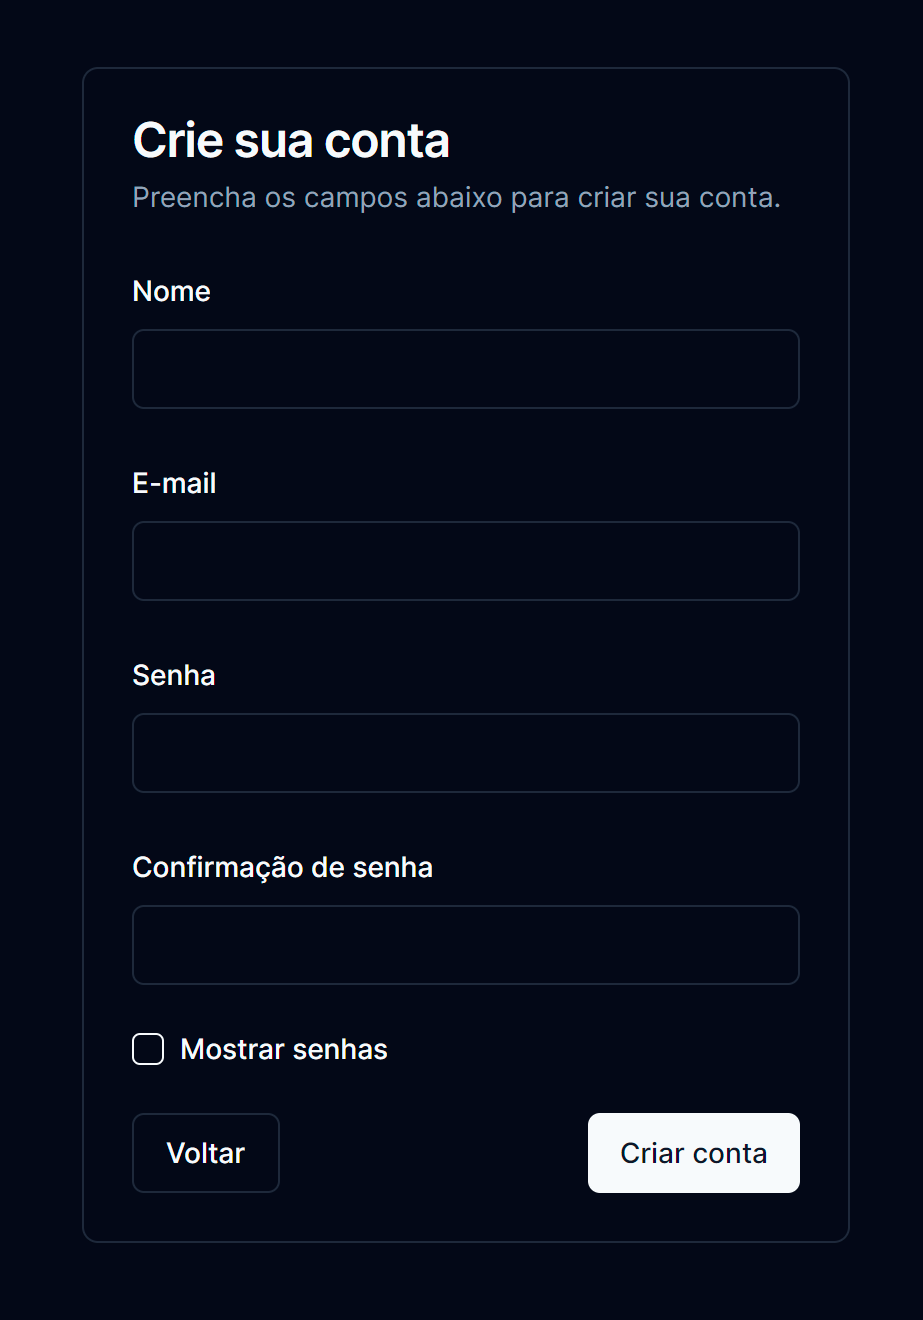
\includegraphics[width=0.8\textwidth]{assets/codeboard/signup-page.png}
    \caption{Página de cadastro da plataforma Codeboard UERJ.}
    \label{fig:signup-page}
\end{figure}

Durante o processo de autenticação, a plataforma utiliza tokens de autenticação para manter o usuário autenticado. O token é gerado no servidor e enviado para o cliente, onde é armazenado no navegador por meio de cookies. O token é utilizado para autenticar o usuário em todas as requisições feitas para o servidor, garantindo que o usuário esteja autenticado em todas as páginas da plataforma.

\subsubsection{Gerenciamento de Salas}

A funcionalidade de gerenciamento de salas permite que o professor crie, edite e acesse salas de aula. A criação de uma sala é feita através de um formulário que solicita o nome da sala e a descrição da atividade prática. Após a criação, o professor pode acessar a sala e adicionar alunos a ela.

\begin{figure}[H]
    \centering
    \includegraphics[width=0.8\textwidth]{diagrams/user-room-flow.png}
    \caption{Diagrama do fluxo de gerenciamento de salas.}
    \label{fig:user-room-flow}
\end{figure}

A tela de listagem de salas é a primeira tela exibida ao usuário após o login. Ela exibe todas as salas em que o usuário é dono ou membro. O usuário pode acessar uma sala clicando no botão de acesso, que o redireciona para a tela da sala.

\begin{figure}[H]
    \centering
    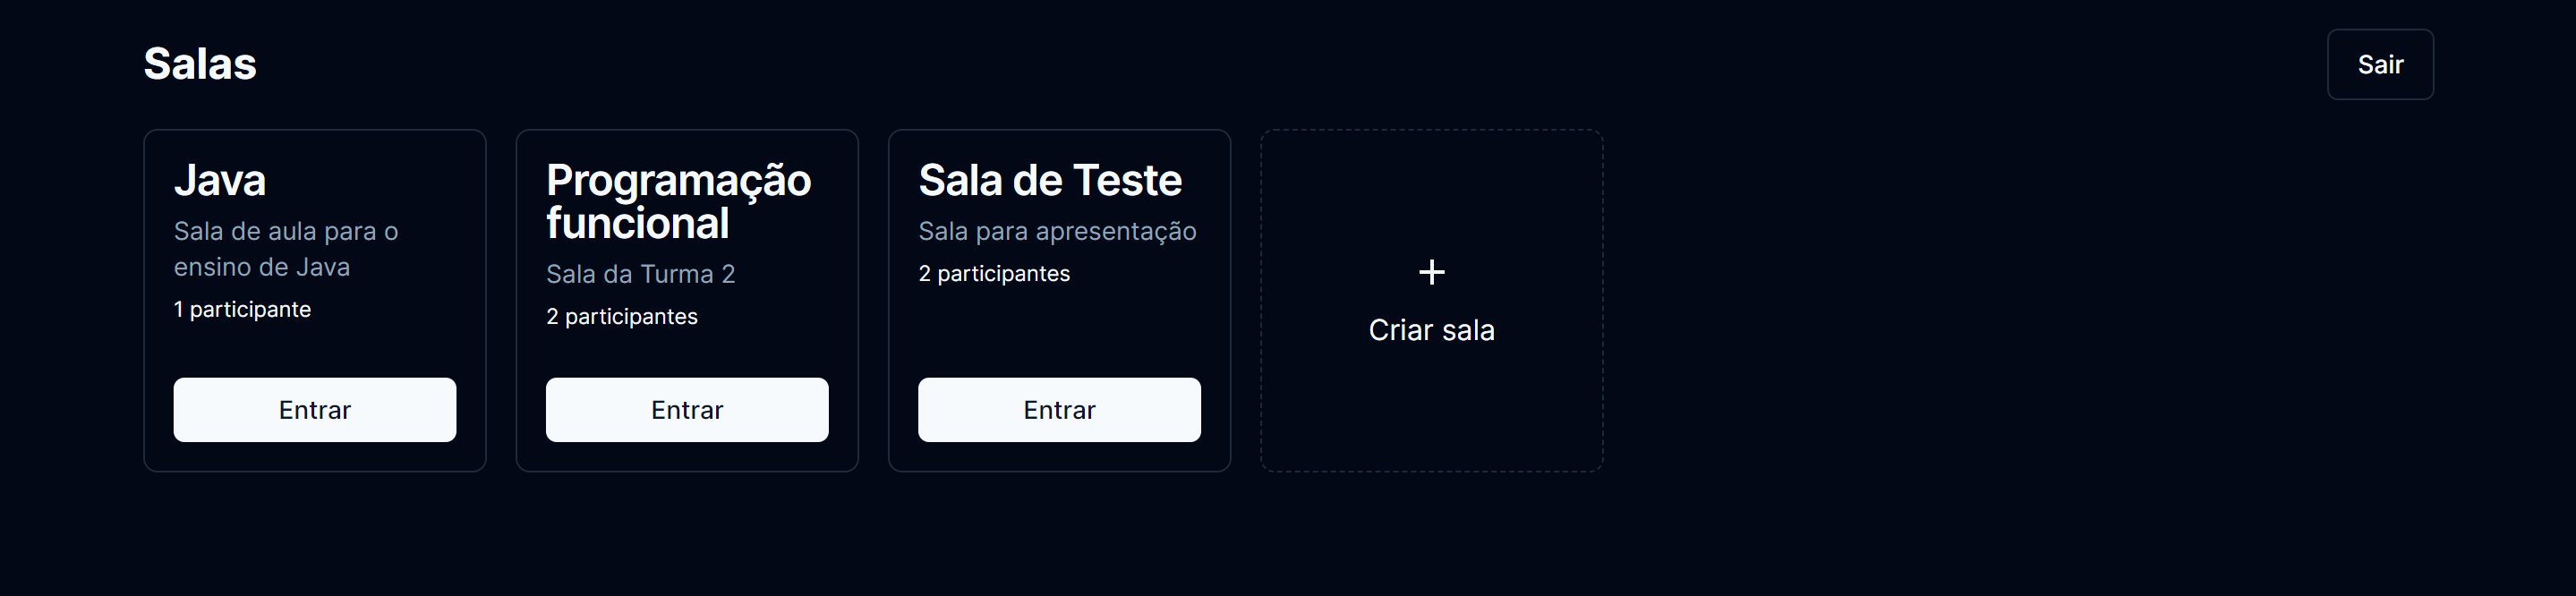
\includegraphics[width=0.8\textwidth]{assets/codeboard/rooms-page.png}
    \caption{Página de listagem de salas da plataforma Codeboard UERJ.}
    \label{fig:rooms-page}
\end{figure}

Nesta mesma tela da figura \ref{fig:rooms-page}, o usuário pode criar uma nova sala clicando no botão de criação de sala. O usuário é redirecionado para uma tela de criação de sala, onde ele pode preencher o nome e a descrição da sala. Após a criação, o usuário é redirecionado para a tela da sala.

\begin{figure}[H]
    \centering
    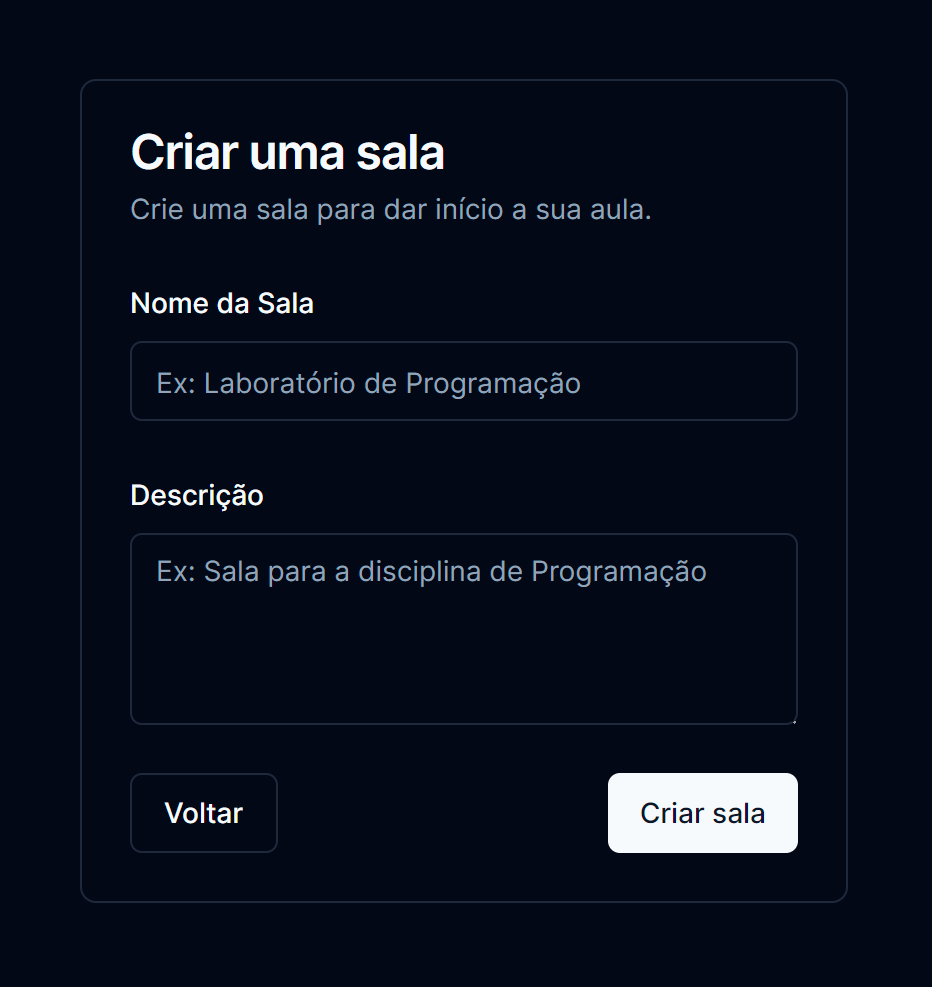
\includegraphics[width=0.8\textwidth]{assets/codeboard/create-room-page.png}
    \caption{Página de criação de sala da plataforma Codeboard UERJ.}
    \label{fig:create-room-page}
\end{figure}

Para adicionar alunos à sala, o usuário pode clicar num botão de adição de participantes representado por um ícone de usuário. A plataforma exibe um modal com um campo de e-mail, onde o usuário pode informar o e-mail do aluno que deseja adicionar à sala. Após a adição, o aluno se torna membro da sala e pode acessá-la.

\begin{figure}[H]
    \centering
    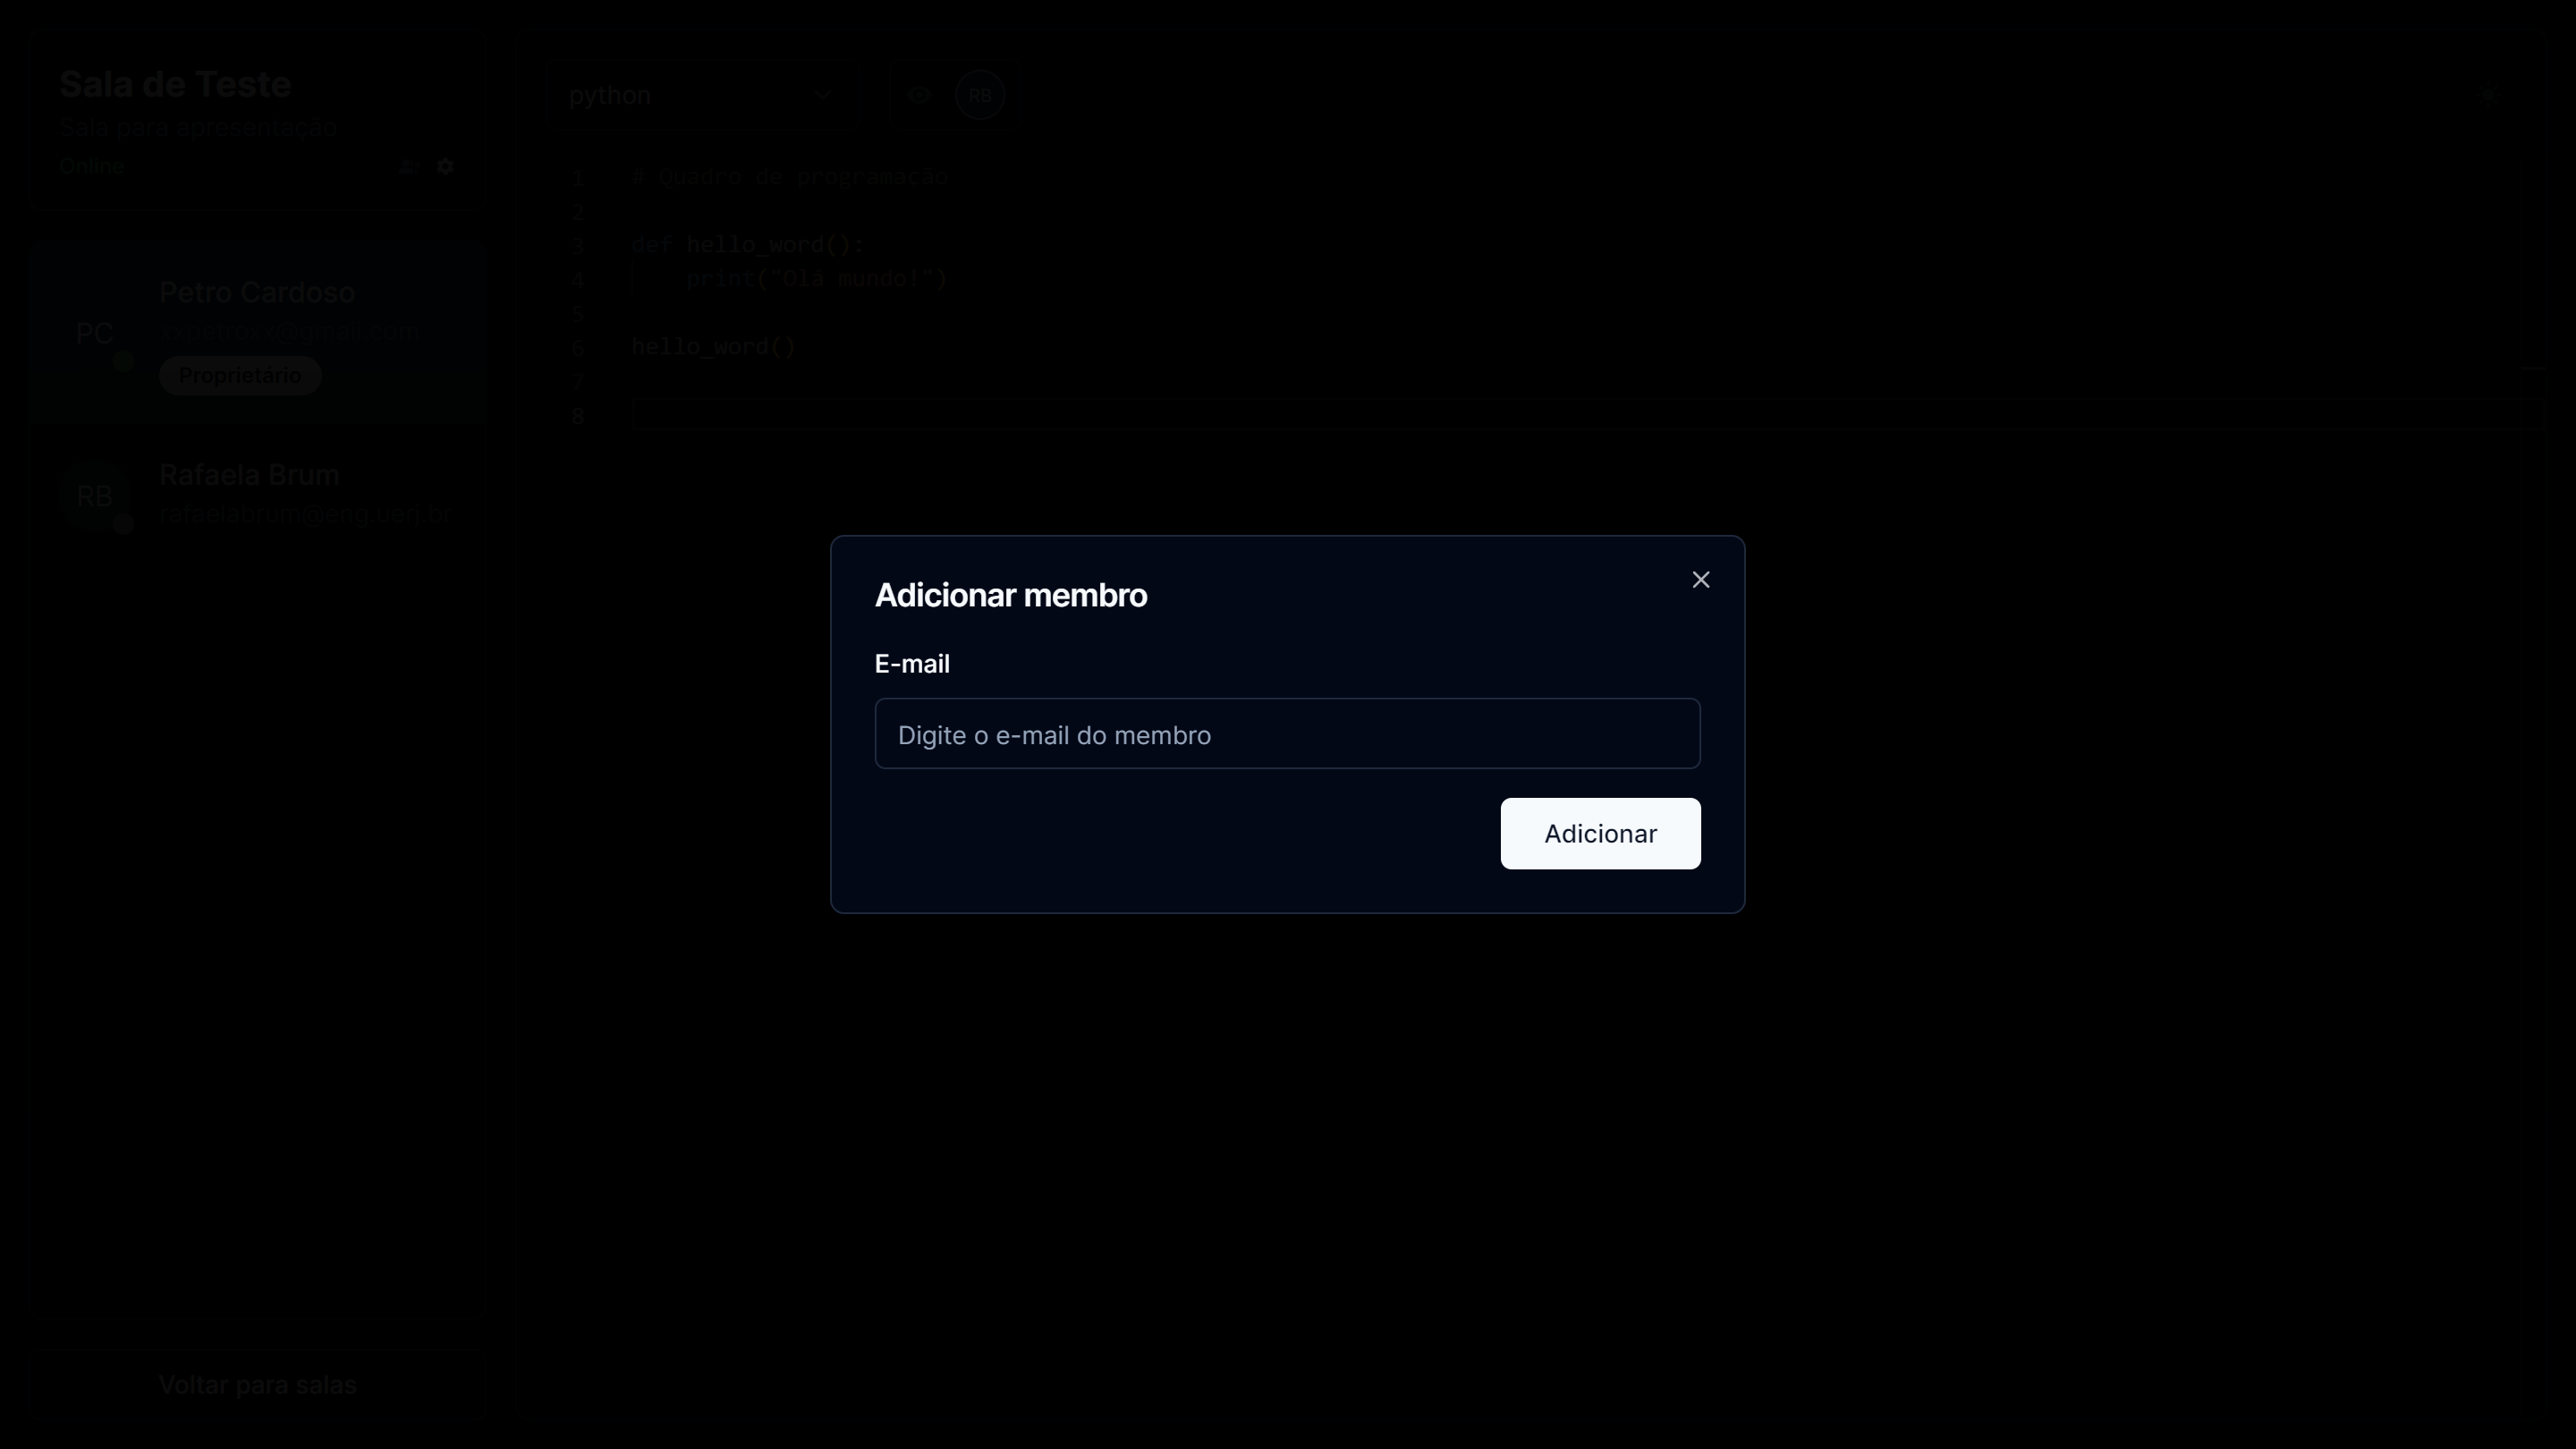
\includegraphics[width=0.8\textwidth]{assets/codeboard/add-member-modal.png}
    \caption{Página de adição de alunos à sala da plataforma Codeboard UERJ.}
    \label{fig:add-member-modal}
\end{figure}

\subsubsection{Quadro de Programação em Tempo Real}

A funcionalidade de quadro de programação em tempo real é a principal funcionalidade da plataforma. Ela permite que os alunos escrevam códigos de programação diretamente no navegador, sem a necessidade de instalar um ambiente de desenvolvimento integrado (IDE).

Para acessar o quadro de programação, o usuário deve acessar a sala desejada. A plataforma exibe uma tela dividida em dois módulos, o módulo lateral de seleção de usuário e o módulo central de edição de código.

\begin{figure}[H]
    \centering
    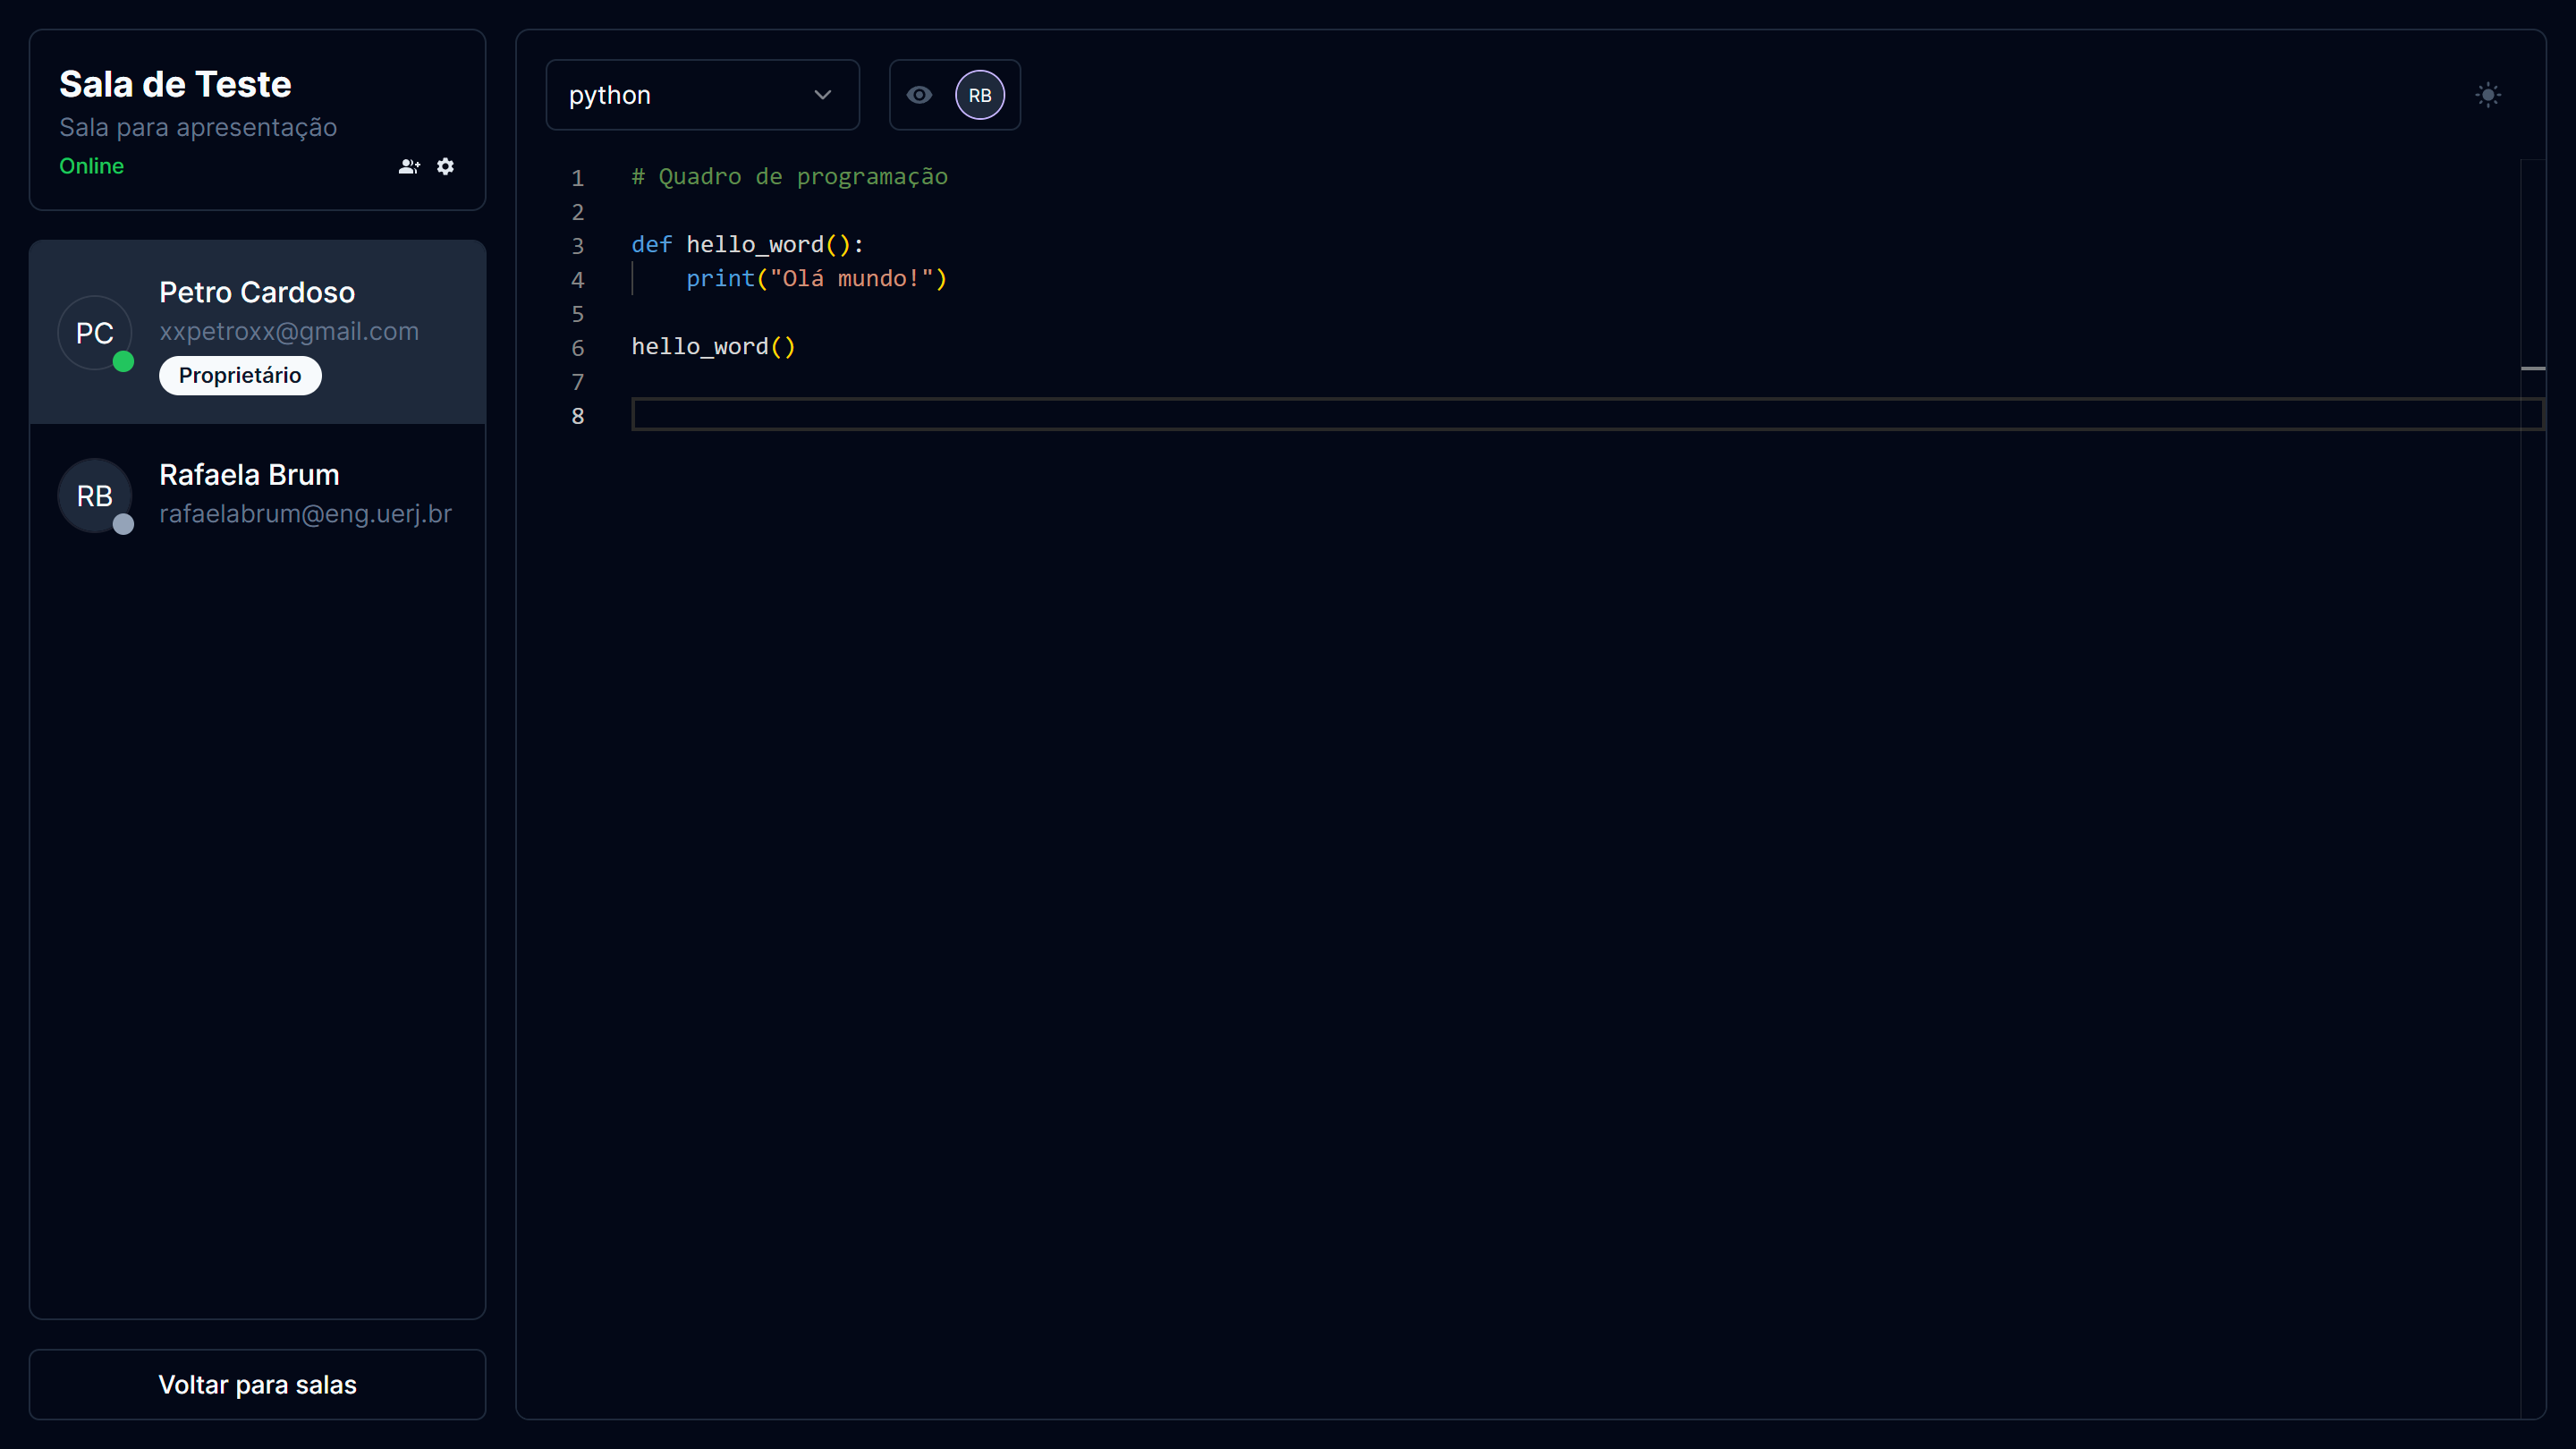
\includegraphics[width=0.8\textwidth]{assets/codeboard/room-details-page.png}
    \caption{Página da sala de programação da plataforma Codeboard UERJ.}
    \label{fig:room-details-page}
\end{figure}


Como mostra a figura \ref{fig:room-details-page}, o módulo lateral exibe a lista de participantes da sala. Para cada membro listado, é exibido o nome, a foto de perfil e indicadores para caso ele esteja online ou esteja editando o seu próprio código. O usuário pode selecionar outro membro da sala na lista lateral para visualizar e interagir com o código dele.

Caso o usuário já esteja com si mesmo selecionado, ele poderá editar o próprio código, trocar de linguagem de programação e visualizar quem está visualizando seu código. O código é salvo automaticamente a cada edição realizada pelo usuário.

Acima do módulo lateral, a plataforma exibe o nome da sala e sua descrição. Caso o usuário seja o dono da sala, também serão exibidos os botões de adição de participantes e de configuração da sala. O botão de adição de participantes permite que o usuário adicione novos participantes à sala, enquanto o botão de configuração permite que o usuário edite o nome e a descrição da sala.

\begin{figure}[H]
    \centering
    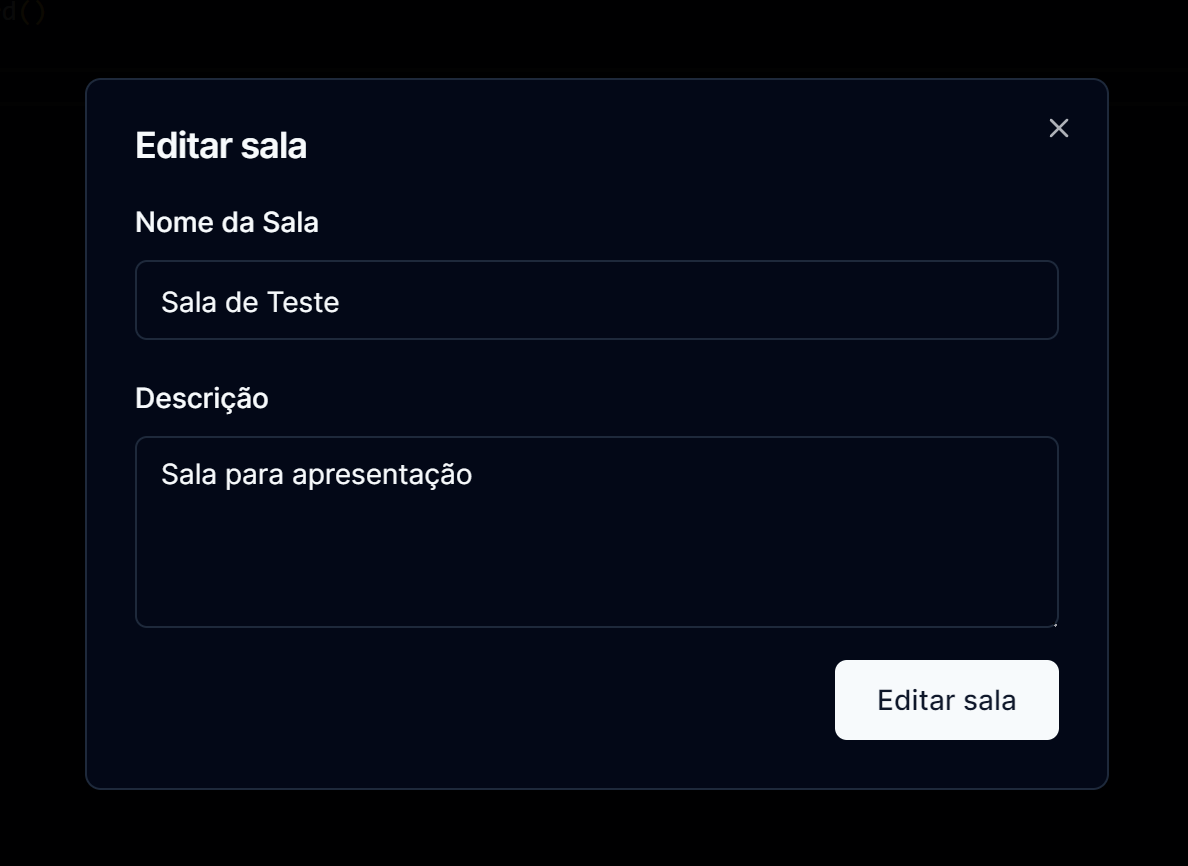
\includegraphics[width=0.8\textwidth]{assets/codeboard/edit-room-modal.png}
    \caption{Modal de configuração de sala da plataforma Codeboard UERJ.}
    \label{fig:edit-room-modal}
\end{figure}


Abaixo do módulo lateral, a plataforma exibe um botão de saída da sala. Ao clicar neste botão, o usuário é redirecionado para a tela de listagem de salas, onde ele pode acessar outras salas ou criar uma nova sala.

O módulo central exibe o editor de código. Este editor suporta as funcionalidades básicas de um IDE, como coloração de sintaxe, auto-completar e formatação de código. Durante a visualização do código de outro usuário, o usuário pode somente fazer marcações que são exibidas em tempo real para o outros usuários presentes no quadro.

\begin{figure}[H]
    \centering
    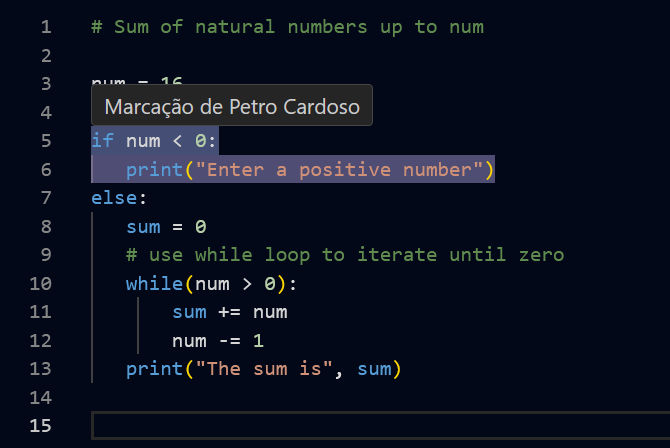
\includegraphics[width=0.8\textwidth]{assets/codeboard/code-editor-user-highlight.png}
    \caption{Marcação de código na plataforma Codeboard UERJ.}
    \label{fig:code-editor-user-highlight}
\end{figure}

Na parte superior do editor, o usuário pode selecionar a linguagem de programação desejada. A plataforma suporta as linguagens de programação mais utilizadas, como C, C++, Java, Python, JavaScript, entre outras. A seleção da linguagem de programação altera a coloração de sintaxe do editor, facilitando a escrita e a leitura do código.

\begin{figure}[H]
    \centering
    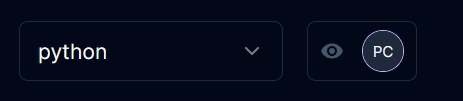
\includegraphics[width=0.8\textwidth]{assets/codeboard/code-editor-toolbar.png}
    \caption{Barra de ferramentas do editor de código da plataforma Codeboard UERJ.}
    \label{fig:code-editor-toolbar}
\end{figure}

Ao lado da seleção de linguagem, o usuário pode visualizar quem está visualizando o seu código no momento. A plataforma exibe uma lista horizontal com estes visualizadores, permitindo que ele saiba quem está acompanhando o seu progresso.


\subsubsection{Regras de Negócio}

Existem algumas regras de negócio que devem ser seguidas para garantir o bom funcionamento da plataforma. Estas regras são implementadas no backend da plataforma e são responsáveis por validar os dados dos usuários e das salas, bem como garantir a segurança e a integridade dos dados.

\paragraph{Autenticação}

\begin{itemize}
    \item \textbf{Cadastro de Usuários}: A plataforma deve fornecer um mecanismo de cadastro de usuários que permita aos usuários se registrarem na plataforma. Para isso, é necessário solicitar os dados dos usuários, como nome, e-mail e senha, e armazená-los de forma segura e protegida no banco de dados.
    \item \textbf{Validação de Dados}: A plataforma deve garantir que os dados dos usuários sejam válidos e consistentes. Para isso, é necessário validar os dados dos usuários durante o processo de cadastro e login e garantir que os dados sejam consistentes e íntegros.
    \item \textbf{Proteção de Dados}: A plataforma deve garantir que os dados dos usuários sejam protegidos e seguros. Para isso, é necessário armazenar os dados dos usuários de forma segura e protegida, utilizando técnicas de criptografia e hash de senhas.
    \item \textbf{Login de Usuários}: A plataforma deve garantir que somente usuários cadastrados possam fazer login. Para isso, é necessário verificar se o e-mail e a senha informados são válidos durante o processo de login e gerar um token de autenticação para manter o usuário autenticado.
    \item \textbf{Gerenciamento de Sessões}: A plataforma deve garantir que as sessões dos usuários sejam gerenciadas de forma segura e eficiente. Para isso, é necessário gerar tokens de autenticação para manter os usuários autenticados e garantir que as sessões sejam encerradas após um período de inatividade.
    \item \textbf{Restrição de Acesso}: A plataforma deve garantir que somente usuários autenticados tenham acesso às funcionalidades da plataforma. Para isso, é necessário verificar se o usuário está autenticado antes de permitir o acesso às funcionalidades.
\end{itemize}

\paragraph{Gerenciamento de Salas}

\begin{itemize}
    \item \textbf{Criação de Salas}: A plataforma deve fornecer um mecanismo de criação de salas que permita aos usuários criarem novas salas. Para isso, é necessário solicitar os dados das salas, como nome e descrição, e armazená-los de forma segura e protegida no banco de dados.
    \item \textbf{Validação de Dados}: A plataforma deve garantir que os dados das salas sejam válidos e consistentes. Para isso, é necessário validar os dados das salas durante o processo de criação e edição e garantir que os dados sejam consistentes e íntegros.
    \item \textbf{Restrição de Acesso}: A plataforma deve garantir que somente participantes da sala tenham acesso à ela. Para isso, é necessário verificar se o usuário é dono ou membro da sala antes de permitir o acesso à sala.
    \item \textbf{Gerenciamento de Participantes}: A plataforma deve fornecer um mecanismo de adição e remoção de participantes que permita aos usuários gerenciarem os participantes das salas. Para isso, é necessário verificar se o usuário é dono da sala antes de permitir a adição ou remoção de participantes.
    \item \textbf{Restrição de Edição}: A plataforma deve garantir que somente o dono da sala possa editar os dados da sala. Para isso, é necessário verificar se o usuário é dono da sala antes de permitir a edição dos dados da sala.
\end{itemize}

\paragraph{Quadro de Programação}

\begin{itemize}
    \item \textbf{Editor em Tempo Real}: A plataforma deve fornecer um mecanismo de edição de código em tempo real que permita aos usuários escrever códigos de programação diretamente no navegador. Para isso, é necessário implementar um editor de código que suporte as funcionalidades básicas de um IDE, como coloração de sintaxe, auto-completar e formatação de código.
    \item \textbf{Restrição de Escrita}: A plataforma deve garantir que não haja conflitos de escrita durante a edição do código em tempo real. Para isso, é necessário implementar um mecanismo de bloqueio de escrita que permita que somente o proprietário do código possa editá-lo.
    \item \textbf{Marcação de Código}: A plataforma deve fornecer um mecanismo de marcação de texto que permita aos usuários visualizarem e interagirem com o código de outros usuários. Para isso, é necessário implementar um mecanismo de marcação que exiba as alterações em tempo real para os outros usuários presentes no quadro.
    \item \textbf{Seleção de Linguagem}: A plataforma deve fornecer um mecanismo de seleção de linguagem que permita aos usuários escolher a linguagem de programação desejada. Para isso, é necessário implementar um seletor de linguagem que altere a coloração de sintaxe do editor de código.
    \item \textbf{Visualização de Usuários}: A plataforma deve fornecer um mecanismo de visualização de usuários que permita aos usuários saber quem está visualizando o seu código. Para isso, é necessário implementar uma lista de visualizadores que exiba os usuários presentes no quadro.
\end{itemize}

\paragraph{Lista de Participantes}

\begin{itemize}
    \item \textbf{Visualização de Participantes}: A plataforma deve fornecer um mecanismo de visualização de participantes que permita aos usuários saber quem está presente na sala. Para isso, é necessário implementar uma lista de participantes que exiba os usuários presentes na sala.
    \item \textbf{Indicadores de Presença}: A plataforma deve fornecer um mecanismo de indicação de presença que permita aos usuários saber quem está online e quem está editando o código. Para isso, é necessário implementar indicadores de presença que exibam se o usuário está online e se está editando o código.
    \item \textbf{Seleção de Participantes}: A plataforma deve fornecer um mecanismo de seleção de participantes que permita aos usuários visualizarem e interagirem com o código de outros participantes. Para isso, é necessário implementar um seletor de participantes que permita selecionar o participante desejado.
\end{itemize}


\subsection{Arquitetura da Plataforma}
% Revisado

Nesta seção, será apresentada a arquitetura da plataforma Codeboard UERJ. A plataforma é estruturada em três camadas principais: o backend, o banco de dados e o frontend. Cada uma dessas camadas desempenha um papel específico na plataforma, sendo responsável pelas regras de negócio, o armazenamento de dados e a interface com o usuário, respectivamente.

\subsubsection{Backend}
% Revisado

O backend da plataforma é responsável pela implementação das regras de negócio da aplicação. Ele é composto por um servidor NodeJS que utiliza dois métodos de comunicação: REST API e WebSockets. A REST API é usada para comunicação assíncrona entre o cliente e o servidor, enquanto os WebSockets são utilizados para permitir a comunicação em tempo real entre os usuários.

\begin{figure}[H]
    \centering
    \includegraphics[width=0.75\textwidth]{diagrams/backend-architecture.png}
    \caption{Arquitetura do backend da plataforma Codeboard UERJ.}
    \label{fig:backend-architecture}
\end{figure}

Conforme a arquitetura do backend ilustrada na Figura \ref{fig:backend-architecture}, a comunicação entre o cliente e o servidor ocorre através de duas interfaces principais: REST API e WebSockets. A REST API fornece um conjunto de rotas que permitem ao cliente acessar funcionalidades da plataforma, como autenticação de usuários, gerenciamento de salas e edição de código. Os WebSockets, por sua vez, são utilizados para viabilizar a comunicação em tempo real entre os usuários, possibilitando a edição colaborativa de código.


\subsubsection{Banco de Dados NoSQL}
% Revisado

A plataforma utiliza o MongoDB como banco de dados, um sistema NoSQL orientado a documentos. O MongoDB foi escolhido por sua flexibilidade, capacidade de escalabilidade horizontal e eficiência no armazenamento de grandes volumes de dados. Além disso, sua integração simples com o NodeJS o torna uma escolha natural para a plataforma Codeboard UERJ.

O banco de dados é organizado em duas coleções principais: a coleção de usuários e a coleção de salas. A coleção de usuários armazena informações dos usuários cadastrados na plataforma, como nome, e-mail e senha. Já a coleção de salas guarda os dados das salas criadas pelos usuários, incluindo nome, descrição e participantes.

\begin{figure}[H]
    \centering
    \includegraphics[width=0.7\textwidth]{diagrams/database-schema.png}
    \caption{Esquema do banco de dados da plataforma Codeboard UERJ.}
    \label{fig:database-schema}
\end{figure}

Conforme o esquema do banco de dados ilustrado na Figura \ref{fig:database-schema}, a coleção "User", responsável por armazenar os dados dos usuários, inclui os seguintes campos:

\begin{table}[H]
    \centering
    \begin{tabular}{|c|c|c|c|}
        \hline
        \textbf{Campo} & \textbf{Descrição}             & \textbf{Tipo} & \textbf{Obrigatório} \\
        \hline
        \_id           & Identificador único do usuário & ObjectId      & Sim                  \\
        name           & Nome do usuário                & String        & Sim                  \\
        email          & E-mail do usuário              & String        & Sim                  \\
        password       & Hash da senha do usuário       & String        & Sim                  \\
        createdAt      & Data de criação do usuário     & Date          & Sim                  \\
        \hline
    \end{tabular}
    \caption{Campos da coleção "User" do banco de dados da plataforma Codeboard UERJ.}
    \label{tab:user-collection-fields}
\end{table}

É importante destacar que a coleção de usuários possui um campo "password" que armazena o hash da senha do usuário. Essa prática é adotada por motivos de segurança, garantindo que a senha do usuário não seja armazenada em texto puro no banco de dados, o que poderia expor as informações dos usuários em caso de vazamento de dados.

A coleção "Room", responsável por armazenar os dados das salas, contém os seguintes campos:

\begin{table}[H]
    \centering
    \begin{tabular}{|c|c|c|c|}
        \hline
        \textbf{Campo} & \textbf{Descrição}             & \textbf{Tipo}   & \textbf{Obrigatório} \\
        \hline
        \_id           & Identificador único da sala    & ObjectId        & Sim                  \\
        name           & Nome da sala                   & String          & Sim                  \\
        description    & Descrição da sala              & String          & Não                  \\
        owner          & Identificador do dono da sala  & ObjectId        & Sim                  \\
        members        & Lista de participantes da sala & Array<ObjectId> & Não                  \\
        createdAt      & Data de criação da sala        & Date            & Sim                  \\
        \hline
    \end{tabular}
    \caption{Campos da coleção "Room" do banco de dados da plataforma Codeboard UERJ.}
    \label{tab:room-collection-fields}
\end{table}


Podemos observar que a coleção de salas possui os campos "owner" e "members" que armazenam os identificadores do dono e dos participantes da sala, respectivamente. Estes campos são utilizados para estabelecer a relação entre os usuários e as salas.

A coleção "Board", responsável por armazenar os dados dos quadros de programação, contém os seguintes campos:

\begin{table}[H]
    \centering
    \begin{tabular}{|c|c|c|c|}
        \hline
        \textbf{Campo} & \textbf{Descrição}             & \textbf{Tipo} & \textbf{Obrigatório} \\
        \hline
        \_id           & Identificador único do quadro  & ObjectId      & Sim                  \\
        user         & Identificador do usuário dono do quadro & ObjectId      & Sim                  \\
        room         & Identificador da sala do quadro & ObjectId      & Sim                  \\
        language       & Linguagem de programação       & String        & Sim                  \\
        content           & Código de programação          & String        & Sim                  \\
        updatedAt      & Data da última atualização      & Date          & Não                  \\
        createdAt      & Data de criação      & Date          & Sim                  \\
        \hline
    \end{tabular}
    \caption{Campos da coleção "Board" do banco de dados da plataforma Codeboard UERJ.}
    \label{tab:board-collection-fields}
\end{table}

A coleção de "Board" possui os campos "user" e "room" que armazenam os identificadores do usuário dono do quadro e da sala do quadro, respectivamente. Esses campos são utilizados para estabelecer a relação entre os usuários, as salas e os quadros de programação.


Embora o banco de dados seja NoSQL, a plataforma Codeboard UERJ adota um esquema de dados bem definido para assegurar a consistência e a integridade das informações. Esse esquema é estabelecido no backend da plataforma com o auxílio do pacote "mongoose", que simplifica a modelagem dos dados e a interação com o banco de dados MongoDB.

\subsubsection{Comunicação Síncrona via REST API}
% Revisado

A REST API é formada por um conjunto de rotas que possibilitam ao cliente acessar as funcionalidades da plataforma. Essas rotas são implementadas com o framework ExpressJS, que facilita a criação de rotas e middlewares em aplicações NodeJS.

Na REST API, existem três tipos principais de rotas: de autenticação, de usuários e de salas. As rotas de autenticação são responsáveis pela criação e autenticação de usuários, enquanto as rotas de usuários permitem o acesso e a atualização dos dados dos usuários. Já as rotas de salas são utilizadas para criar, acessar e gerenciar as salas.

\begin{table}[H]
    \centering
    \begin{tabular}{|c|c|c|c|}
        \hline
        \textbf{Método} & \textbf{Rota}                  & \textbf{Descrição}            & \textbf{Autenticação} \\
        \hline
        GET             & /api/health                    & Verifica o status do servidor & Não                   \\
        \hline
        POST            & /api/auth/signup               & Cadastra um novo usuário      & Não                   \\
        POST            & /api/auth/login                & Autentica um usuário          & Não                   \\
        \hline
        GET             & /api/user                      & Retorna os dados do usuário   & Sim                   \\
        PUT             & /api/user                      & Edita os dados do usuário     & Sim                   \\
        \hline
        GET             & /api/rooms                     & Lista todas as salas          & Sim                   \\
        POST            & /api/rooms                     & Cria uma nova sala            & Sim                   \\
        GET             & /api/rooms/:id                 & Retorna uma sala específica   & Sim                   \\
        PUT             & /api/rooms/:id                 & Edita uma sala específica     & Sim                   \\
        POST            & /api/rooms/:id/members         & Adiciona um membro à sala     & Sim                   \\
        DELETE          & /api/rooms/:id/members/:userId & Remove um membro da sala      & Sim                   \\
        \hline
    \end{tabular}
    \caption{Rotas da REST API da plataforma Codeboard UERJ.}
    \label{tab:rest-api-routes}
\end{table}


\subsubsection{Sistema de Autenticação}
% Revisado

As rotas descritas na tabela \ref{tab:rest-api-routes} que requerem autenticação, são protegidas por um middleware que verifica se o usuário está autenticado antes de permitir o acesso. A autenticação do usuário na plataforma é realizada através de um token, que é gerado no servidor e enviado ao cliente após o login. 

O token de autenticação é gerado utilizando o pacote "jsonwebtoken", que implementa o padrão JWT (JSON Web Token). A escolha do JWT como mecanismo de autenticação foi motivada pela necessidade de suportar a infraestrutura horizontal da plataforma, que facilita a escalabilidade e a distribuição dos servidores. Como o JWT é um mecanismo stateless, não é necessário armazenar o estado da sessão no servidor. Isso o torna ideal para aplicações distribuídas e escaláveis, pois o estado da sessão é armazenado no próprio token, que é enviado ao cliente.

O token é criado com base no ID do usuário e uma chave secreta, que é mantida nos servidores. Esse token é assinado com a chave secreta e enviado ao cliente, onde é armazenado no navegador por meio de cookies. A cada requisição feita ao servidor, o token é utilizado para autenticar o usuário, garantindo sua autenticidade em todas as páginas da plataforma.

O token de autenticação tem um tempo de expiração configurado no servidor. Após esse período, o token é invalidado, e o usuário é automaticamente desconectado da plataforma.

\subsubsection{Banco de Dados Chave-Valor}
% Revisado

A plataforma Codeboard UERJ utiliza um banco de dados chave-valor para armazenar informações temporárias, como a lista de usuários online, o código dos quadros de programação e a lista de visualizadores dos quadros. Esse banco de dados é implementado com o Redis, um sistema de armazenamento em memória de código aberto.

A escolha do Redis como banco de dados chave-valor foi motivada por sua eficiência, alto desempenho na manipulação de dados em memória e capacidade de escalabilidade horizontal. O Redis é amplamente utilizado em aplicações que demandam alta disponibilidade e baixa latência, características importantes para a plataforma Codeboard UERJ.


\begin{table}[H]
    \centering
    \begin{tabular}{|c|p{6cm}|c|}
        \hline
        \textbf{Namespace}                   & \textbf{Descrição}                       & \textbf{Expiração} \\
        \hline
        room:\{roomId\}:users                & Lista de ID dos usuários online          & 1 dia              \\
        \hline
        board:\{roomId\}:\{boardId\}:code    & Código do quadro de programação          & 1 dia              \\
        \hline
        board:\{roomId\}:\{boardId\}:viewers & Lista de ID dos visualizadores do quadro & 1 dia              \\ 
        
        \hline
    \end{tabular}
    \caption{Estrutura do banco de dados chave-valor da plataforma Codeboard UERJ.}
    \label{tab:key-value-database}
\end{table}

Conforme a estrutura do banco de dados chave-valor ilustrada na Tabela \ref{tab:key-value-database}, o Redis é utilizado para armazenar informações temporárias relacionadas à comunicação em tempo real. Os dados são organizados em namespaces que representam diferentes contextos da aplicação, como salas, quadros de programação e visualizadores. Cada namespace possui um tempo de expiração configurado no servidor, assegurando que os dados sejam automaticamente removidos após um período de inatividade.

A remoção automática dos dados é importante para garantir a integridade e a eficiência do banco de dados chave-valor. Como esses dados são temporários e não precisam ser armazenados por longos períodos, a expiração dos dados permite liberar recursos e manter o banco de dados limpo e organizado.

\subsubsection{Comunicação Síncrona em Tempo Real}

% TODO 
% - Falar sobre a comunicação em tempo real com WebSockets
% - Falar sobre middlewares de autenticação
% - Explicar namespaces e rooms
% - Listar eventos que são emitidos e ouvidos e suas respectivas funções
%   - connection
%   - room:join
%   - room:joined
%   - room:members
%   - board:join
%   - board:joined
%   - board:viewers
%   - board:leave
%   - board:left
%   - board:write
%   - board:typed
%   - board:written
%   - board:highlight
%   - board:highlighted
%   - board:read
%   - disconnecting
% - Criar diagrama de sequência da comunicação em tempo real, com um exemplo de interação entre os usuários

\subsubsection{Comunicação Assíncrona utilizando Filas}

% TODO
% Falar sobre worker e filas


\subsubsection{Frontend}

To do
